% last updated in April 2002 by Antje Endemann
% Based on CVPR 07 and LNCS, with modifications by DAF, AZ and elle, 2008 and AA, 2010, and CC, 2011; TT, 2014; AAS, 2016

\documentclass[runningheads]{llncs}
\usepackage{graphicx}
\usepackage{amsmath,amssymb} % define this before the line numbering.
\usepackage{ruler}
\usepackage{color}
\usepackage[width=122mm,left=12mm,paperwidth=146mm,height=193mm,top=12mm,paperheight=217mm]{geometry}
\begin{document}
% \renewcommand\thelinenumber{\color[rgb]{0.2,0.5,0.8}\normalfont\sffamily\scriptsize\arabic{linenumber}\color[rgb]{0,0,0}}
% \renewcommand\makeLineNumber {\hss\thelinenumber\ \hspace{6mm} \rlap{\hskip\textwidth\ \hspace{6.5mm}\thelinenumber}}
% \linenumbers
\pagestyle{headings}
\mainmatter
\def\ECCV16SubNumber{***}  % Insert your submission number here

\title{A view-invariant compositional hierarchical representation of 3D shape} % Replace with your title

\titlerunning{ECCV-16 submission ID \ECCV16SubNumber}

\authorrunning{ECCV-16 submission ID \ECCV16SubNumber}

\author{Draft for anonymous ECCV submission}
\institute{Paper ID \ECCV16SubNumber}


\maketitle

\begin{abstract}
We propose a novel view-invariant compositional hierarchical
representation of 3D shapes.


 \keywords{Compositional Hierarchies}
\end{abstract}


\section{Introduction}

Several compositional hierarchical representations for 2D contour
shapes have been proposed in
\cite{Leonardis1,aktas2014graph,Ommer}. Some important
properties of this type of representations have been reported in literature, such as scalability, sub-linear
growth of representations with respect to the number of object categories, fast
inference and matching, reusability of shape parts within and across
the categories which leads to compactness of the representations and
enables transfer of knowledge between objects and categories.

Relatively little work has been done in the domain of the 3D
compositional part-based models. Classical work of Biederman was
done in 80s \cite{biederman1987recognition}. He has shown that
people are able to recognize objects by dividing them into geons,
which are the main components objects that form objects. In his approach.
geons are based on a set of standard geometric primitives (e.g.
cylinders, cones), which are assembled to form object and
category models.

There exist several more recent methods in this domain. Wessel and
Klein \cite{pratikakis2010learning} presented a feature selection
technique, which decomposes 3D objects into sections that can be
represented by planes, spheres, cylinders, cones and tori.
They introduced a probabilistic framework modeling the spatial
arrangements between these shape primitives.

Early work of Biederman \cite{biederman1987recognition}, Wessel and Klein \cite{pratikakis2010learning} both use a set of pre-defined shapes as simple primitives with very shallow hierarchical structures, which makes it difficult to generalise over complex shapes. In contrast, our methodology is entirely data-driven, and is able to learn structures of arbitrary size and complexity. 

More recently, neural networks have been used in creating 3D representations \cite{wu20153d,Su_2015_ICCV}. Wu et al. \cite{wu20153d} proposed a 3D hierarchical compositional
framework called 3D-ShapeNet. They present a 3D model
as a probability distribution of binary variables on a 3D voxel
grid, using a convolutional Deep Belief Network (DBN). They demonstrated
ability of their approach to recognize object categories from range
images and complete full 3D shape of objects. Similarly, Su et al. \cite{Su_2015_ICCV} have applied convolution neural
networks to 3D shape recognition problem. They first perform recognition
of objects presented from a single view, and then present a novel
CNN architecture that combines information from multiple views of each object into a single compact descriptor.

Hu and Zhu \cite{hu2015learning} presented a framework for learning
of 3D templates from 3D models of cars using AND-OR trees. They used
the learned templates for simultaneous object detection,
localization and pose estimation. This method exploits the well-defined 3D structure of cars to learn 3D compositions, which would otherwise be a combinatorial problem. It requires manual annotation of object parts, hence addition of a new category is difficult. Our approach does not require annotation of object parts, and is able to find recurring patterns in data automatically. Finally, methods based on deep learning \cite{wu20153d,Su_2015_ICCV} perform well on object categorization tasks. The challenge lies in designing the network to different tasks, since it is not possible to visualise the learned features in order to check if they are visually meaningful. 

\section{Representation\label{sec:Representation}}

\subsection{Definitions\label{sec:Definitions}}

Our representation of 3D surface shapes is a \textbf{compositional
hierarchical shape vocabulary}. The hierarchy contains several
layers $L_n, n\,{\geqslant}\,1,$ each of which comprises a set of
elements called \textbf{parts} representing various 3D surfaces. The
first layer $L_1$ contains only one part representing the small
disk-shaped planar surface, while parts of the higher layers
describe larger and more complex surfaces.

A part $P_{i}^n$ of the layer $L_n$, $\forall n\,{>}\,1$ is a
composition of \textbf{subparts}, i.e. parts of the previous layer
$L_{n-1}$. It describes a distribution of possible relative
positions and relative orientations of these constituent subparts,
thus exerting a curtain degree of shape variability. Each vocabulary
part contains its own frame of reference in which relative positions
and orientations of subparts are defined.

\textbf{Part realization} $R$ is an instance of a part detected in
the data. Part realizations for all layers $n\,{>}\,1$ have their
own frames of reference which are aligned with the Darboux frame of
the underlying surface, i.e. the surface normal $N$ and principal
directions $T_1, T_2$. The frame of references of vocabulary parts
and part realizations can be converted from one to another in SE3.

\subsection{Properties of the representation\label{sec:Properties}}

One of the properties of our the compositional hierarchical
representation of 3D shape is \textbf{view and rotational
invariance} of parts. Part index encodes shape properties only, and
does not change with change of object's pose or with change of the
viewing angle. This property is achieved by describing all spatial
relations of subparts relatively to other parts, while frames of
reference for part realizations are attached to the Darboux frames
of surfaces. Any rigid body transformation of objects does not
change the relative spatial relation of objects' parts.

Next property of our representation is \textbf{scalability}, i.e. a
sub-linear growth of the vocabulary size with a number of object
categories. This property is achieved because of re-usability of
parts across different categories.

Another property of our framework in \textbf{redundancy} of the
explanations provided by the part realizations. We start inference
of vocabulary parts on each data point (e.g. at each pixel) on the
object surface. This usually results in lots of part realizations
with overlapping receptive fields.

Next property is \textbf{flexibility} of compositions parts. In each
vocabulary part positions and orientations of the sub-parts are
parameterized by the Gaussian distributions encoding a certain
degree of shape variability.


\section{Learning of the vocabulary\label{sec:Learning}}

The vocabulary learning procedure comprises several steps. Assume we
are learning the vocabulary of the layer $L_n$.

\subsection{Collecting of co-occurrence statistics\label{sec:Collection}}
    The first step is the collection of co-occurrence statistics of parts of the layer $L_{n-1}$ in the training data. At
    this stage, we learn statistical maps for each pair of parts ($P_i^{n-1}$, $P_j^{n-1}$) of the layer
    $L_{n-1}$. Statistical maps are functions $f_{i,j}(x,y,z,q_1,q_2,q_3,q_4)$ which give number of observations of realizations of the part
    $P_j^{n-1}$ at the relative position $p = [x,y,z]$ and relative orientation described
    by the quaternion $q = [q_1,q_2,q_3,q_4]$ w.r.t. realizations of the part
    $P_i^{n-1}$. Statistical maps describe co-occurrences of parts only within a local geodesic neighborhood (called \textbf{receptive
    field}) of each part. The receptive fields grow with each subsequent
    layer.

    Positions and orientations are described in the frame of reference
    of the part $P_i^{n-1}$, which is referred as a \emph{reference sub-part}
    in this context. To process statistical maps faster, we make them discrete, i.e. we define steps
    for $p$ and $q$, thus partitioning the receptive field into
    bins. Each co-occurrence observed in the training
    data increases the count for the relevant bin.

    It is important to mention, that the term \emph{relative orientation}
    has a different meaning for different layers of the hierarchy. Assume
    we are describing the relative orientation of the part $P_j^{n-1}$ w.r.t the central sub-part
    part $P_i^{n-1}$. For the layers $n\,{<}\,5$ the quaternion $q$ describes
    the rotation that transforms the surface normal of part $P_i^{n-1}$ into the surface normal
    of the part $P_j^{n-1}$. For the higher layers the quaternion
    describes the
    transformation that is required to rotate the full reference frame of the part $P_i^{n-1}$ to the
    frame of the part $P_j^{n-1}$, i.e. in the higher layers the quaternions are computed from
    directional cosine matrices.

    We make this difference because: a) lower layer parts usually represent relatively small
    surface patches that resemble planar surfaces, b) at the lower layers
    quality of the input data may have a significant influence due to noise,
    discretization and meshing properties; that is why robust estimation of the principal
    directions of curvatures may be problematic. We find it is enough to
    describe the
    relative orientations of normals for the lower layers and then
    switch to description of relative orientations of reference frames for higher layers.



\subsection{Clustering of the statistical maps\label{sec:Clustering}}

Clustering of the statistical maps is performed to obtain a set of
pairs (doublets). It is performed in four steps:

\begin{itemize}
    \item Assume, that we have a list of size $m$ of non-empty bins. Each bin $B_i$ is
    characterized by the average relative position $p_i = [x,y,z]$ and the average quaternion $q_i = [q_1,q_2,q_3,q_4]$ representing
    the relative orientation.
    \item Compute the distance matrix $D$ of size $m \times m$,
    which defines distances between each pair of bins.
    The distance $D_{hk} = d_{ER}(B_h, B_k)$ between two bins $B_h$ and $B_k$ is defined as follows:
    \begin{align}
        d_{ER}(B_h, B_k) = d_E(p_h, p_k) + \alpha \, d_R(q_h, q_k),
    \end{align}
    %\[ d_{ER}(B_h, B_k) = d_E(p_h, p_k) + \alpha d_R(q_h, q_k), \]
    where $d_E(\cdot,\cdot)$ is the Euclidean distance between
    bins' positions and $d_R(\cdot,\cdot)$ is a rotational distance
    between quaternions $q_h$ and $q_k$.
    The rotational distance is defined as
    \begin{align}
        d_r(q_h, q_k) = \sqrt{1 - q_h \, q_k}.
    \end{align}

    All quaternions must be normalized before computing the distance
    matrix. Similar distance measures are discussed in
    \cite{kuffner2004effective}.
    \item Apply hierarchical agglomerative clustering using the distance
    matrix D. To find the best number of clusters we use a
    modified Davies\,--\,Bouldin index. In the original work the Davies\,--\,Bouldin
    index is defined as follows \cite{davies1979cluster}:

    \begin{align}
    DB = \frac{1}{n}\sum\limits_{i=1}^{n} \max\limits_{i \neq j}^{} \left(\frac{\sigma_i + \sigma_j}{d(c_i, c_j)}\right),
    \end{align}

 %   \[ DB = \frac{1}{n}\sum\limits_{i=1}^{n} \max\limits_{i \neq j}^{} \left(\frac{\sigma_i + \sigma_j}{d(c_i, c_j)}\right), \]
    where $\sigma_x$ is s the average distance of all bins in cluster x
    to centroid $c_x$, and $d(c_i,c_j)$ is the distance between centroids $c_i$ and
    $c_j$.
    In our framework two degenerate cases may appear where this index
    becomes ill-defined: a) when there is only one bin in a cluster ($\sigma_x$ can not be
    defined), b) when the statistical map can be fit with one cluster
    ($d(c_i, c_j)$ can not be defined). To avoid these
    problems we introduce an additional constraint specifying maximal size of
    clusters. The results of clustering on the statistical maps are shown in
    Figure \ref{fig:clustering}.

    \item Parameterize each cluster with two Gaussians. One of them (3 dimensional) represents
variance of the relative positions, and another one (4 dimensional)
represents variance of the relative orientations. That means for
each cluster $k$ we compute $\mu_{E_k}$, $\Sigma_{E_k}$, $\mu_{q_k}$
and $\Sigma_{q_k}$. Note, that since the statistical maps are
defined for each pair of parts ($P_i^{n-1}$, $P_j^{n-1}$) of the
layer $L_{n-1}$, a set of clusters described by the parameters
$\mu_E$, $\Sigma_E$, $\mu_q$ and $\Sigma_q$ is different for each
pair ($P_i^{n-1}$, $P_j^{n-1}$).
\end{itemize}

\begin{figure}
\centering
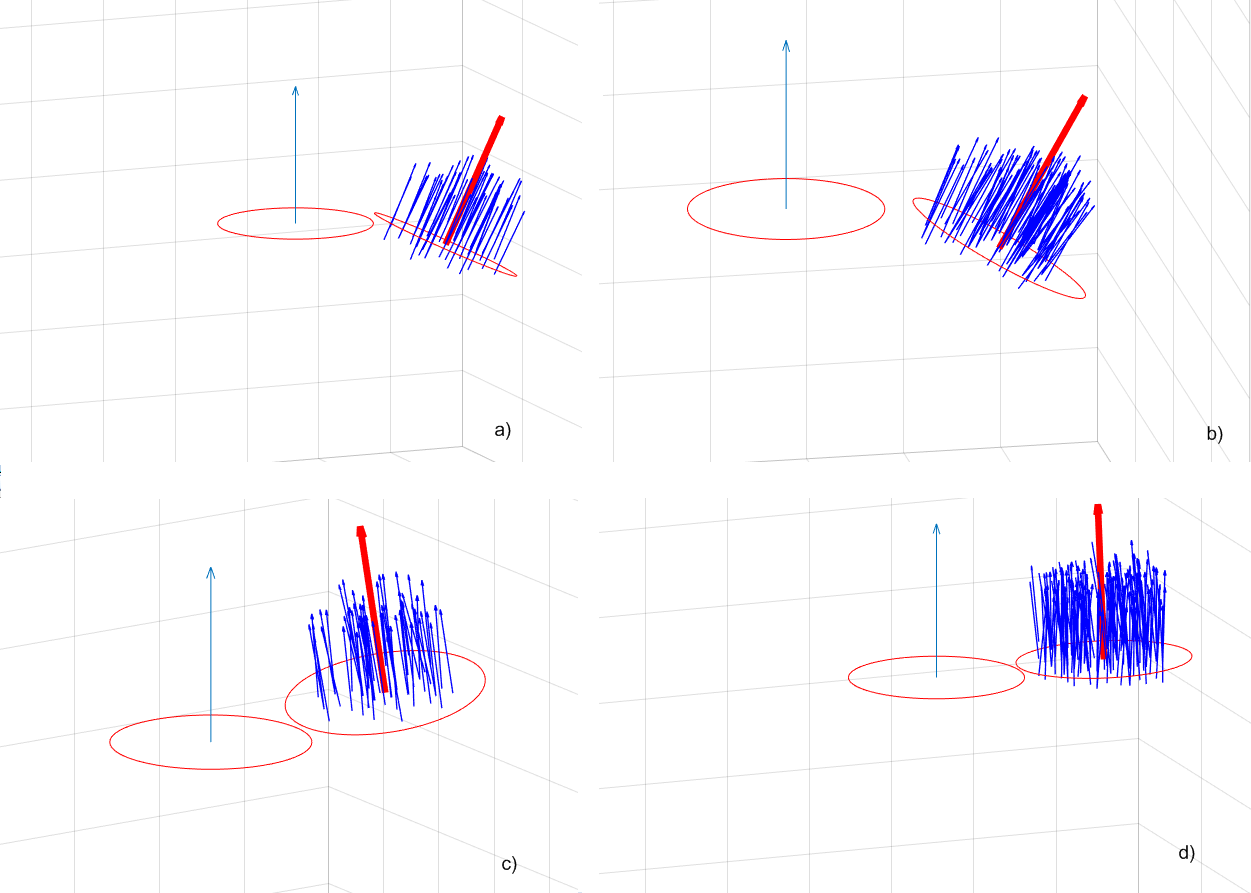
\includegraphics[scale=0.3]{Clustering}
\caption{The statistical map is clustered into four clusters. Circle
in the middle shows the reference part. Blue arrows show positions
and orientations represented by the non-empty bins of the
statistical map, that were assigned to one of the clusters. Circles
of the right define a sub-part which is located in the mean position
and mean orientation of the cluster. Bold red arrow defines normal
of this part.} \label{fig:clustering}
\end{figure}

These steps result in a set of doublets which are then used to build
triples which form the vocabulary of the layer $L_n$, $\forall
n\,{>}\,1$.

\subsection{Form a set of candidate parts \label{sec:Candidates}}

Assume we have a set of doublets after clustering of the statistical
maps. It often happens that there are two or more doublets that
exist simultaneously within the same receptive field. We measure the
probabilities of joint observation of two doublets fully within a
receptive field. Those combinations of pairs which have
probabilities above a pre-defined threshold value are included in
the set of candidate parts $\mathcal{C}_n$ for the layer $L_n$.

\subsection{Compression by OR-nodes \label{sec:OR-nodes}}

Some of the candidate parts $\mathcal{C}_n$ for the layer $L_n$ may
represent similar surface types, although represented as
compositions of different subparts. This problem is illustrated in
Figure \ref{fig:OrNodes}, where different spatial arrangements of
different subparts result in the same surface types. In order to
reduce the number of parts and facilitate generalization we perform
compression by introducing OR-nodes. Each of these nodes
accommodates several candidate parts from $\mathcal{C}_n$ which
represent similar surface types.

\begin{figure}
\centering
\includegraphics[scale=0.6]{OrNode}
\caption{Similar surface types are achieved as compositions of
different subparts, or different spatial arrangements of the same
sub-parts.} \label{fig:OrNodes}
\end{figure}

We use the \textbf{volume between two surfaces} to measure the
similarities of parts $P_i^n$ and $P_j^n$ from $\mathcal{C}_n$. The
volume is measured when the frames of references of these parts are
aligned, i.e. the centres of parts are in the same location, and the
axes are pointing in the same direction. We call this distance
between parts $d_v(P_i^n, P_j^n)$.

\section{Inference\label{sec:Inference}}

Once learning from a training data set has occurred we wish to infer
the existence of parts on a new example objects. The goal of
inference is to find activations (realizations) of vocabulary parts
in the input data. Inference can be done from depth images, point
clouds, or triangulated mesh models. The general inference pipeline
remains the same for all data types, however, some implementation
details differ depending on the type of input data.

Our algorithm starts with inference from the first layer, and then
subsequently infers parts for the higher layers (bottom-up
inference) growing the receptive field size and matching
combinations of part realizations in each receptive field against
vocabulary parts of the next layer. We start inference at each data
point, (e.g. at each pixel in the case of depth images), thereby
obtaining many part realizations with overlapping receptive fields.

Inference of the first layer realizations is performed on three
different scales. As the first layer part is a disk-shaped planar
patch, we perform inference of planar patches of three different
radii. For instance, a relatively large planar surface patch can be
expressed either as the first layer realization of larger radius, or
as a composition of the first layer realizations of a smaller radii.
We have chosen the second way as it gives a more compact
representation and helps to reduce inference time.

In the following we first describe how to perform inference of the
first layer on a single scale, and then describe multi-scale
inference.

\subsection{Inference of the first layer from a single scale\label{sec:InferenceFirstSingle}}

Assume we infer the first layer realizations on the scale $S_i$.
Scale defines the radii of surface patches to be tested for
planarity, let's assume that scale $S_i$ corresponds to the radius
$rad_i$. The algorithm for inference looks as follows:

\begin{enumerate}
\item Define a geodesic receptive field of a radius $rad_i$ around each data point $\rho_i$.
\item Extract all other data points that reside in this
receptive field.
\item Perform a planarity test. This test differs depending
on the data type. For point clouds or range images we perform least
square fitting for these points; for mesh models where surface
normals are available we measure the spread of normal directions
around the direction of the normal at the point $\rho_i$. Based on
the error value (or spread value) we make a decision about the
planarity of the surface patch. If the planarity of the surface is
not confirmed, we stop inference at the point $\rho_i$, otherwise we
go to step 4.
\item Estimate a surface normal $N_i$ for this patch. For depth images and point clouds it is
estimated analytically using plane parameters obtained from the
least squares fitting. For mesh models, when surface normals at each
data point are given, we take the average of the normals of all data
point which belong to the patch.
\item If the planarity of a surface patch is confirmed and the surface normal is
estimated, we say we have found a part realization of layer $L_1$.
The position of this part is defined by the position of $\rho_i$,
and the orientation is $N_i$.
\end{enumerate}


\subsection{Inference of the first layer from multiple scales\label{sec:InferenceFirstMultiple}}

Inference of the first layer parts is done at three different
scales, i.e. we try to find planar patches of three different radii
$rad_1 > rad_2 > rad_3$ in the data. We have a general rule: If the
data around a point $\rho_i$ can be fit with a larger planar patch,
then we don't try to fit the smaller patches around this point. In
this manner we automatically search for the most compact
representation of the data across different scales. Assume we have a
set of data points $\Phi$, the multi-scale inference procedure can
be described as follows:

\begin{enumerate}

\item Perform inference (as described in Section
\ref{sec:InferenceFirstSingle}) of part realizations of the largest
radius $rad_1$. We perform inference for each data point $\rho_i$
from the set $\Phi$. Assume that inference was successful for the
set of points $\Psi \subset \Phi$, while it failed for the set
$\Upsilon \subset \Phi$. (Note that $\Phi = \Psi \bigcup \Upsilon$
and $\Psi \bigcap \Upsilon = \emptyset$).

\item Perform inference of part realizations of the
radius $rad_2$ for each data point from the set $\Upsilon$. Assume
inference was successful for some points, however it failed for the
set of points $\Xi \subset \Upsilon$.

\item Perform inference of part realizations of the
radius $rad_3$ for each data point from the set $\Xi$.

\end{enumerate}


\subsection{Inference of the subsequent layers\label{sec:InferenceNext}}

After inference of the layer $L_1$ is finished, we perform inference
for each subsequent next layer. Assume, we perform inference of the
layer $L_n$ given a set $\Lambda$ of realizations of parts of the
previous layer $L_{n-1}$. We do it using the following procedure:

\begin{enumerate}

\item For each part realization $R_i$ from $\Lambda$ define a geodesic receptive
field of radius defined by the layer $n$. Extract all other part
realizations lying within this receptive field (call this set
$\Omega$).

\item If $R_i$ is a realization of the layer $L_1$ part (at any of three scales), its frame of reference is not defined.
Then we go to step 3, otherwise set the reference frame of the
receptive field $F_i$ equal to the reference frame of $R_i$ and go
to step 4.

\item Estimate the frame of reference for this receptive field. The position of $R_i$ defines origin of this
frame. As for the axes, we make them aligned with the Darboux frame,
i.e. the surface normal at this point and the principal directions
of curvature. We use positions of all part realizations from
$\Omega$ to define the tensor of curvature
\cite{taubin1995estimating}. Eigenvectors of this tensor define the
frame of reference $F = [N, T_1, T_2]$ for this receptive field,
where $N$ is a surface normal and $T_1$ and $T_2$ are are principal
directions. If the principal directions can not be estimated, for
example for planar surfaces or around umbilic points, we select
$T_1$ and $T_2$ as arbitrary directions orthogonal to each other and
to the surface normal $N$.

\item Convert all positions and orientations of all part realizations
belonging to the set $\Omega$ from the global reference frame to the
reference frame $F_i$. This conversion makes positions and
orientations \textbf{relative} to $R_i$.

\item Perform matching of duplets. Assume, that $R_i$ is a
realization of the vocabulary part $P_k^{n-1}$. Also assume that the
set $\Omega$ contains realization $R_j$ of the vocabulary part
$P_a^{n-1}$ at the relative position $p_j = [x,y,z]$ and the
relative orientation defined by the quaternion $q_j = [q_1, q_2,
q_3, q_4]$ w.r.t. $R_i$. Extract from the vocabulary of the layer
$L_n$ a set of clusters corresponding to the pair of parts
($P_k^{n-1}$, $P_a^{n-1}$) described by the following parameters:
$\mu_E$, $\Sigma_E$, $\mu_q$ and $\Sigma_q$. (See section
\ref{sec:Clustering} for more detailes). Then we measure the
Mahalanobis distances from the points $p_j$ and $q_j$ to the
clusters. If both distances (for translation and rotation) are
smaller is than pre-defined thresholds, then we have inferred a
duplet. Repetition of this procedure for all realization from the
set $\Omega$ results in a set of inferred duplets in the receptive
field of $R_i$.

\item Perform inference of triples. For each pair of inferred duplets we form a triple which is matched to the
triples in the vocabulary of the layer $L_n$.


\end{enumerate}

\section{Experiments \label{sec:Experiments}}

\subsection{Learning of compositional hierarchical shape vocabulary from the data set of kitchen objects\label{sec:DataSet}}

We used our framework for learning a compositional hierarchical
shape vocabulary form a data set of kitchen objects. The dataset
contains 15 categories of objects, e.g. mugs, plates, jugs, vases,
etc. Figures \ref{fig:parts4} \ref{fig:parts7} \ref{fig:parts8} show
some of the vocabulary parts of different layers of the hierarchy.
\begin{figure}[t!]
\centering
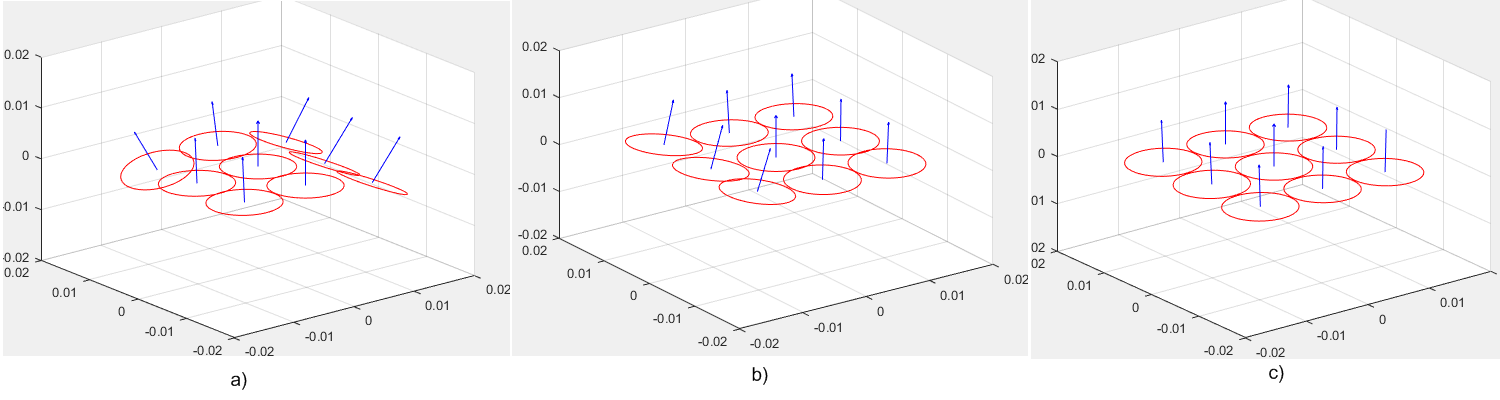
\includegraphics[scale=0.3]{parts4}
\caption{Some parts from the vocabulary of the layer 4}
\label{fig:parts4}
\end{figure}
\begin{figure}[t!]
\centering
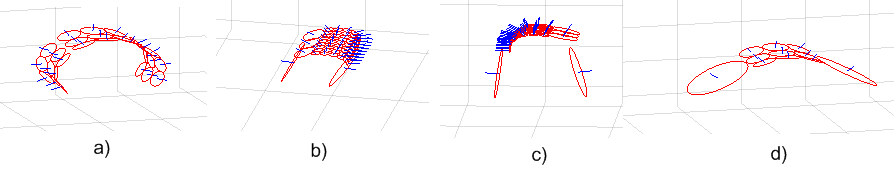
\includegraphics[scale=0.45]{parts7}
\caption{Some parts from the vocabulary of the layer 7}
\label{fig:parts7}
\end{figure}
\begin{figure}[t!]
\centering
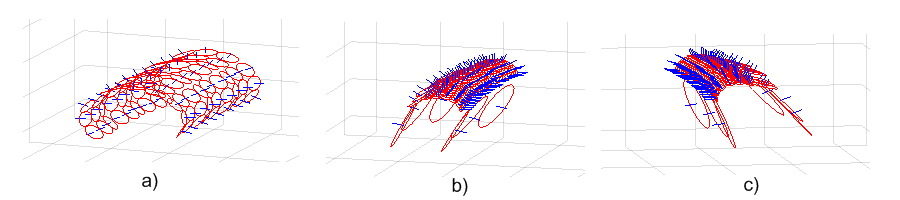
\includegraphics[scale=0.45]{parts8}
\caption{Some parts from the vocabulary of the layer 8}
\label{fig:parts8}
\end{figure}

\subsection{Analysis of the properties of the hierarchy\label{sec:DataSet}}

In this section we analyze properties of our compositional
hierarchy. In particular, we prove its view and rotational and
rotational-invariant properties and share-ability of parts across
categories.

In the first experiment we analyze how the size of the vocabulary
grows with number of object categories. We learn the vocabulary on a
set of objects of a single category. Then we add categories one
after another, and perform vocabulary learning again, measuring size
of the vocabulary of each layer after each iteration. All parameters
and threshold values remain the same.

Figure \ref{fig:scalability} shows the result of this experiment. We
can observe sub-linear growth of the vocabulary size with number of
categories, which is explained by \emph{share-ability} of the
vocabulary parts across categories.

\begin{figure}[t!]
\centering
\includegraphics[scale=0.4]{scalability}
\caption{Number of vocabulary parts learned from subsets comprising
different number of object categories. Left: for the layer 5, Right:
for the layer 6} \label{fig:scalability}
\end{figure}

\section{Conclusions \label{sec:Conclusion}}

We have developed a novel view-invariant framework for learning and
inference of the 3D compositional hierarchical shape vocabulary. So
far we have demonstrated some properties of the framework, such as
view-invariance and scalability, i.e. sub-linear growth of the shape
vocabulary with number of object categories, due to share-ability of
parts.

In the nearest future we aim to demonstrate some other properties of
the framework, for instance ability to predict hidden (occluded)
parts of the objects, and ability to recognize and localize the
objects in the cluttered scenes, and approximately reconstruct their
hidden parts.



\clearpage

\bibliographystyle{splncs}
\bibliography{refs}
\end{document}
